\documentclass{beamer}\usepackage[]{graphicx}\usepackage[]{color}
%% maxwidth is the original width if it is less than linewidth
%% otherwise use linewidth (to make sure the graphics do not exceed the margin)
\makeatletter
\def\maxwidth{ %
  \ifdim\Gin@nat@width>\linewidth
    \linewidth
  \else
    \Gin@nat@width
  \fi
}
\makeatother

\definecolor{fgcolor}{rgb}{0.345, 0.345, 0.345}
\newcommand{\hlnum}[1]{\textcolor[rgb]{0.686,0.059,0.569}{#1}}%
\newcommand{\hlstr}[1]{\textcolor[rgb]{0.192,0.494,0.8}{#1}}%
\newcommand{\hlcom}[1]{\textcolor[rgb]{0.678,0.584,0.686}{\textit{#1}}}%
\newcommand{\hlopt}[1]{\textcolor[rgb]{0,0,0}{#1}}%
\newcommand{\hlstd}[1]{\textcolor[rgb]{0.345,0.345,0.345}{#1}}%
\newcommand{\hlkwa}[1]{\textcolor[rgb]{0.161,0.373,0.58}{\textbf{#1}}}%
\newcommand{\hlkwb}[1]{\textcolor[rgb]{0.69,0.353,0.396}{#1}}%
\newcommand{\hlkwc}[1]{\textcolor[rgb]{0.333,0.667,0.333}{#1}}%
\newcommand{\hlkwd}[1]{\textcolor[rgb]{0.737,0.353,0.396}{\textbf{#1}}}%
\let\hlipl\hlkwb

\usepackage{framed}
\makeatletter
\newenvironment{kframe}{%
 \def\at@end@of@kframe{}%
 \ifinner\ifhmode%
  \def\at@end@of@kframe{\end{minipage}}%
  \begin{minipage}{\columnwidth}%
 \fi\fi%
 \def\FrameCommand##1{\hskip\@totalleftmargin \hskip-\fboxsep
 \colorbox{shadecolor}{##1}\hskip-\fboxsep
     % There is no \\@totalrightmargin, so:
     \hskip-\linewidth \hskip-\@totalleftmargin \hskip\columnwidth}%
 \MakeFramed {\advance\hsize-\width
   \@totalleftmargin\z@ \linewidth\hsize
   \@setminipage}}%
 {\par\unskip\endMakeFramed%
 \at@end@of@kframe}
\makeatother

\definecolor{shadecolor}{rgb}{.97, .97, .97}
\definecolor{messagecolor}{rgb}{0, 0, 0}
\definecolor{warningcolor}{rgb}{1, 0, 1}
\definecolor{errorcolor}{rgb}{1, 0, 0}
\newenvironment{knitrout}{}{} % an empty environment to be redefined in TeX

\usepackage{alltt}

%\setbeamertemplate{background}{\includegraphics[width=\paperwidth,height=\paperheight,keepaspectratio]{ages_background2.png}}

\usepackage[ngerman,english]{babel}
\usepackage{lmodern} % schrift besser lesbar
\usepackage[T1]{fontenc}
\usepackage[utf8]{inputenc}
\usepackage{comment}
\usepackage{colortbl}

\usepackage{amsmath, amsthm}
\usepackage{amssymb}
\usepackage{bbm} % "Blackboard-style" cm fonts

\usepackage[backend = bibtex, natbib = true, style = numeric, sorting = none]{biblatex}
\addbibresource{../../diss_tex/references/mybib.bib}

\usetheme{Boadilla}

%\definecolor{ages}{RGB}{204,164,0}
%\usecolortheme[named=ages]{structure}

\setbeamercovered{transparent}
\beamertemplatenavigationsymbolsempty
\setbeamertemplate{footline}[frame number]

\newcommand\numbered{\setbeamertemplate{footline}[frame number]}
\newcommand\unnumbered{\setbeamertemplate{footline}{}}


\newcommand{\Sin}[1]{\sin\left(#1\right)}%
\newcommand{\Cos}[1]{\cos\left(#1\right)}%
\newcommand{\Log}[1]{\log\left(#1\right)}%
\newcommand{\mli}[1]{\mathit{#1}}% MulitLetterIdentifier - produces nice names for multi character variables in math environments
\IfFileExists{upquote.sty}{\usepackage{upquote}}{}
\begin{document}
\graphicspath{{figures/}}
%\graphicspath{{../../chapters/figures/IPD/}, {../../chapters/figures/}}
%\graphicspath{{D:/diss/chapters/figures/IPD/}} %{{paste0(getwd(), "/chapters/figures/IPD/")}} %{../figures/IPD/}
%% initialize %%



%%%%
\title{Mathematical models in outbreak response}
\subtitle{SE Scientific Communication, 2019}
\author{Lukas Richter}
\date[]{28. June 2019}

% \titlegraphic{
%   
\includegraphics[width=2.0cm]{logo_ages}\hspace*{3cm}~%
%   
\includegraphics[width=2.0cm]{logo_tugraz}
% }

%10-15 min presentation


%%%%%%%%%%%%%%%%%%%%%%%%%%%%%%%%%%%%%%%%%%%%%%
{\unnumbered
\begin{frame}[noframenumbering]
  \titlepage
\end{frame}}
%%%%%%%%%%%%%%%%%%%%%%%%%%%%%%%%%%%%%%%%%%%%%%

%%%%%%%%%%%%%%%%%%%%%%%%%%%%%%%%%%%%%%%%%%%%%%
{\unnumbered
\begin{frame}[noframenumbering]
  \tableofcontents
\end{frame}}
%%%%%%%%%%%%%%%%%%%%%%%%%%%%%%%%%%%%%%%%%%%%%%

\section{Background}
%%%%%%%%%%%%%%%%%%%%%%%%%%%%%%%%%%%%%%%%%%%%%%
\begin{frame}[fragile]{Background}
\begin{center}

\unnumbered
Outbreaks: \\
Influenza, 2009 \\
MERS-Cov (Middle-East Respiratory Syndrome) \\
Ebola, West Africa, DRC \\
Zika Virus, Brazil



\end{center}
\end{frame}
%%%%%%%%%%%%%%%%%%%%%%%%%%%%%%%%%%%%%%%%%%%%%%

%%%%%%%%%%%%%%%%%%%%%%%%%%%%%%%%%%%%%%%%%%%%%%
\begin{frame}[fragile]{Objective/Goal}

during outbreak: \\
exploit all data \\
inform response team in real time \\

in general (also non outbreak situation) \\
allow evidence based decisions \\
compare/assess interventions \\
policy evaluation (before/after in), vaccine programmes \\

track of WHO targets (HIV, HCV)

\end{frame}
%%%%%%%%%%%%%%%%%%%%%%%%%%%%%%%%%%%%%%%%%%%%%%

%%%%%%%%%%%%%%%%%%%%%%%%%%%%%%%%%%%%%%%%%%%%%%
\begin{frame}[fragile]{Types of models}

dynamic, mathematical (SIR) \\
statistical (e.g. Poisson regression) \\
Bayesian statistics \\
spacial stats/models \\

-> visualise outcome

\end{frame}
%%%%%%%%%%%%%%%%%%%%%%%%%%%%%%%%%%%%%%%%%%%%%%


%%%%%%%%%%%%%%%%%%%%%%%%%%%%%%%%%%%%%%%%%%%%%%
\begin{frame}[fragile]{Example of outbreak analytics workflow.}
\begin{center}
\begin{figure}
  \centering
  % \caption{Example of outbreak analytics workflow.}
  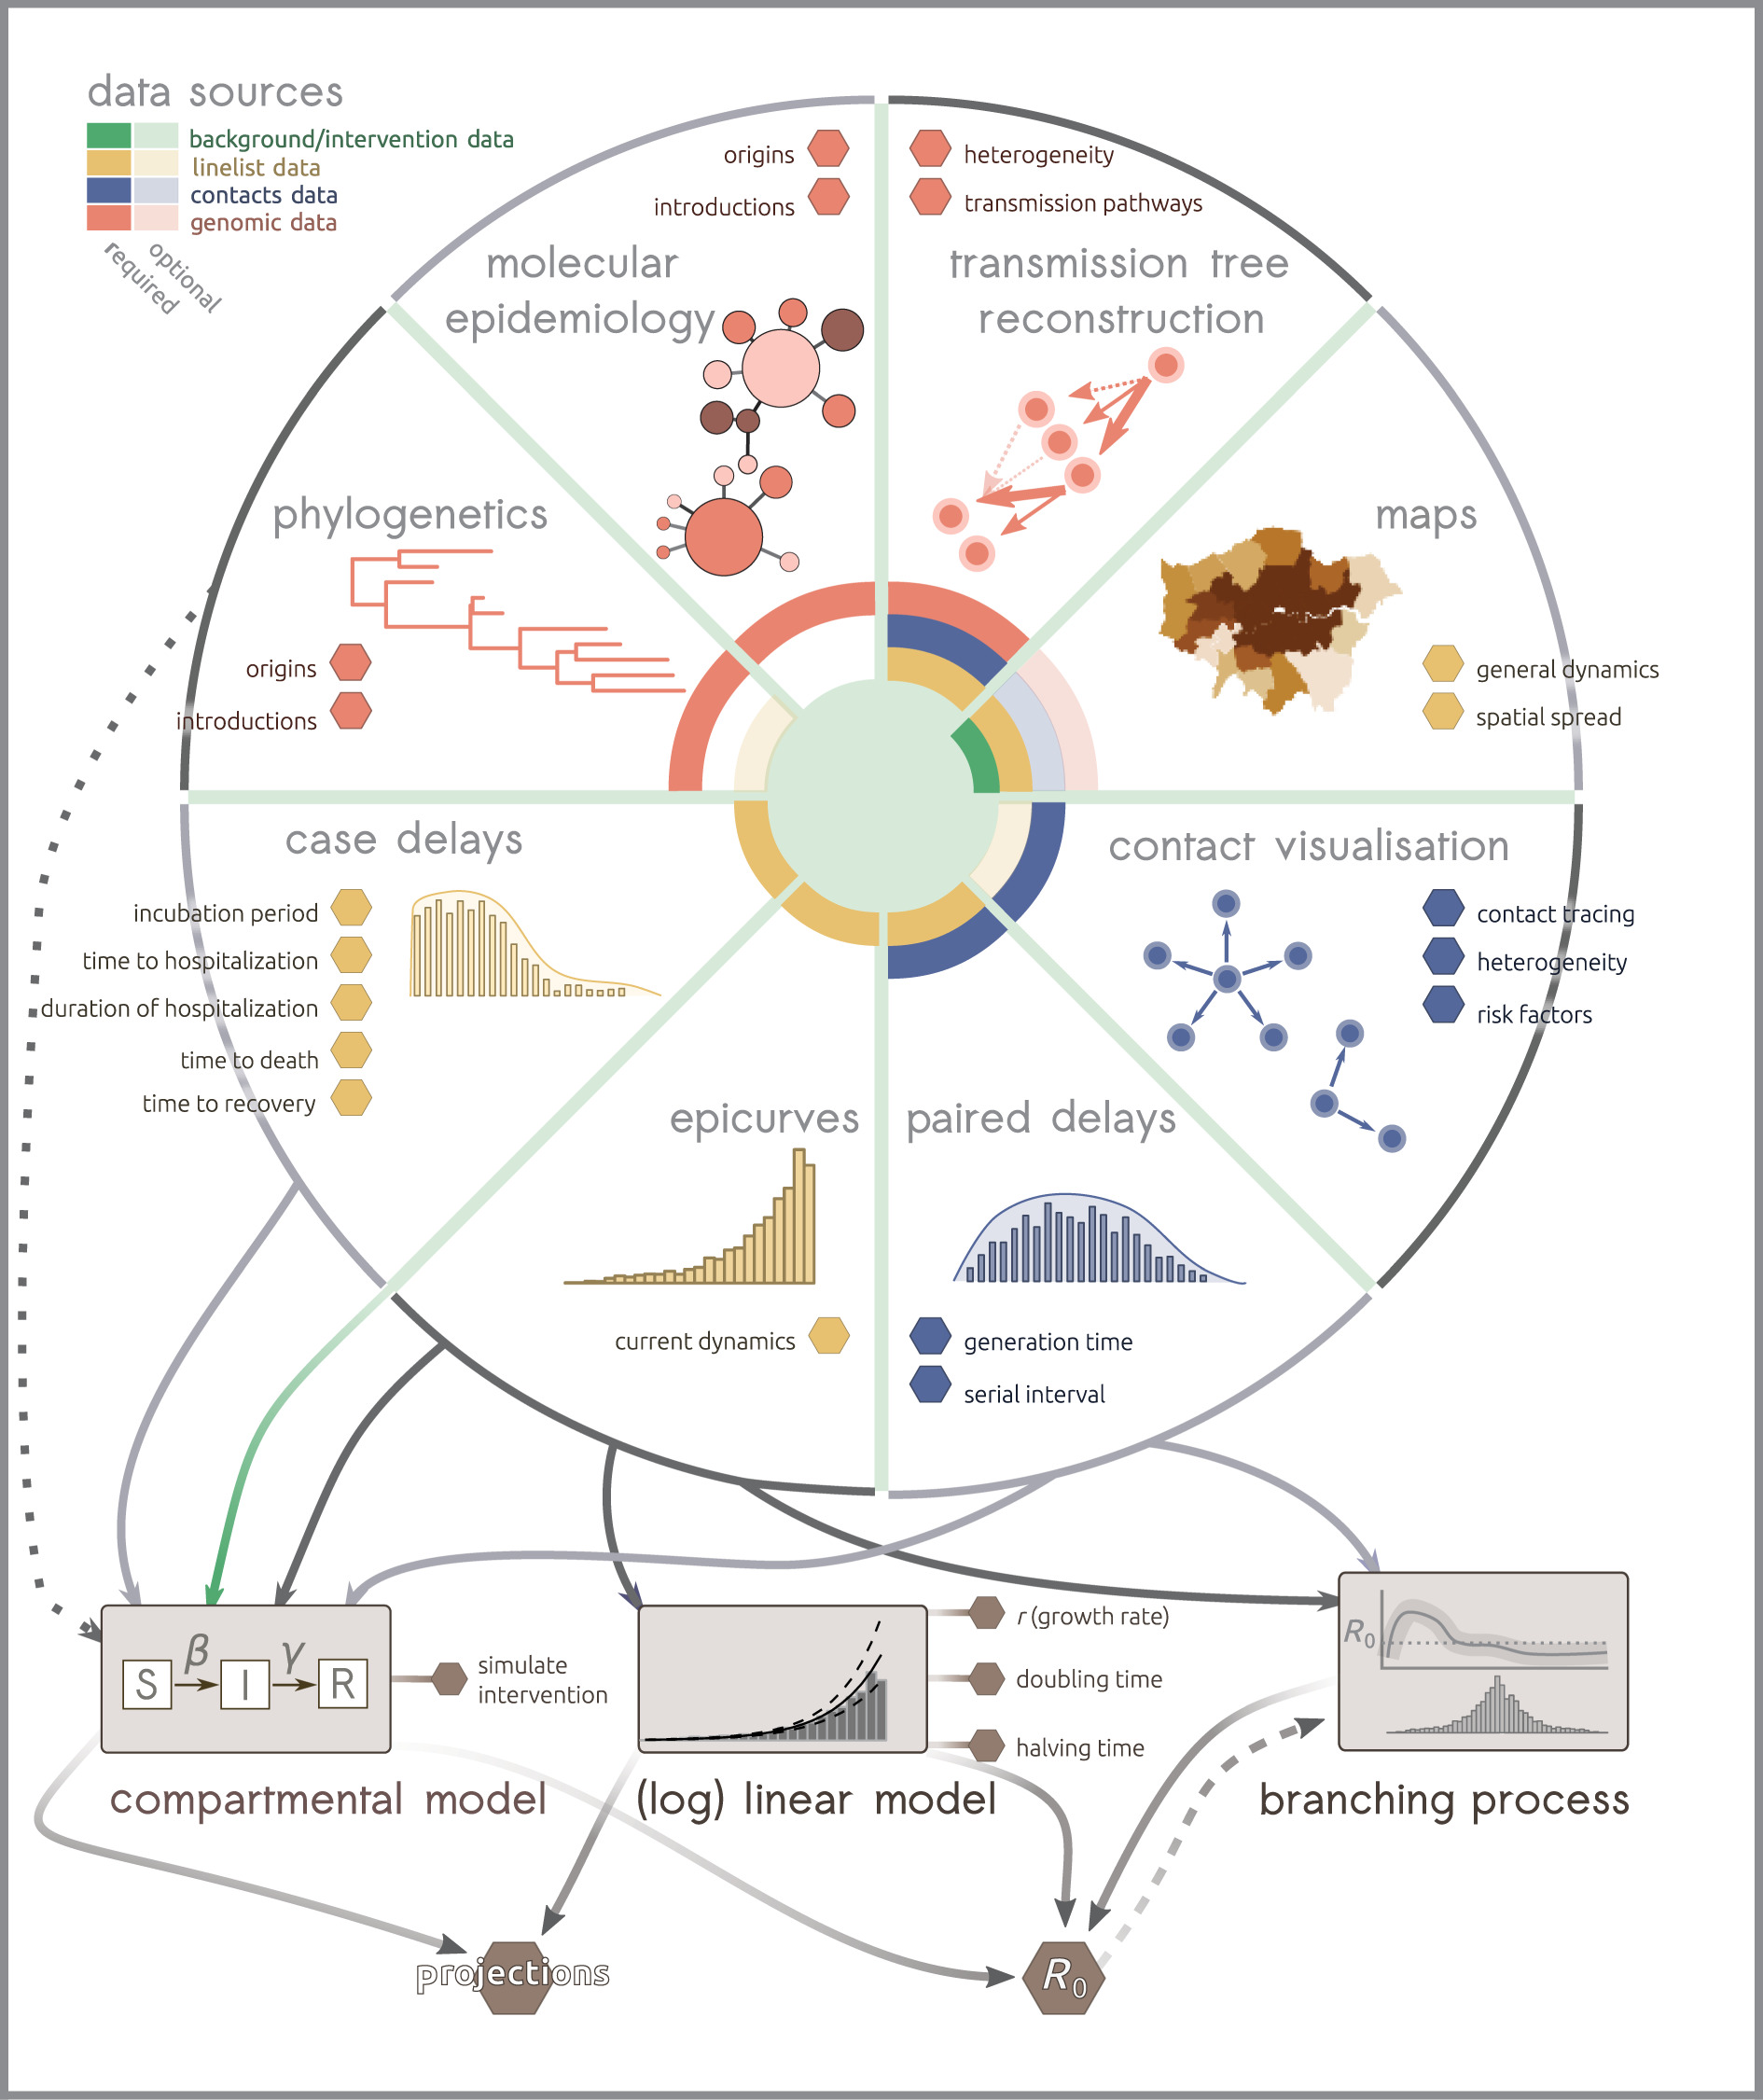
\includegraphics[width=\textwidth,height=0.8\textheight,keepaspectratio]{polonsky2019_Fig2.png}
\end{figure}
\end{center}
\end{frame}
%%%%%%%%%%%%%%%%%%%%%%%%%%%%%%%%%%%%%%%%%%%%%%

%%%%%%%%%%%%%%%%%%%%%%%%%%%%%%%%%%%%%%%%%%%%%%
\begin{frame}[fragile]{IPD}
\begin{center}
\begin{figure}
  \centering
  \caption{Monthly incidence of (A) PCV10 ST-IPD and (B) non-PCV10 ex ST 6A-/19A-IPD, among the $\ge$50 years old, observed and modelled by a segmented negative binominal regression, Austria, January 2009-February 2017, shown are overall and seasonal trends.}
  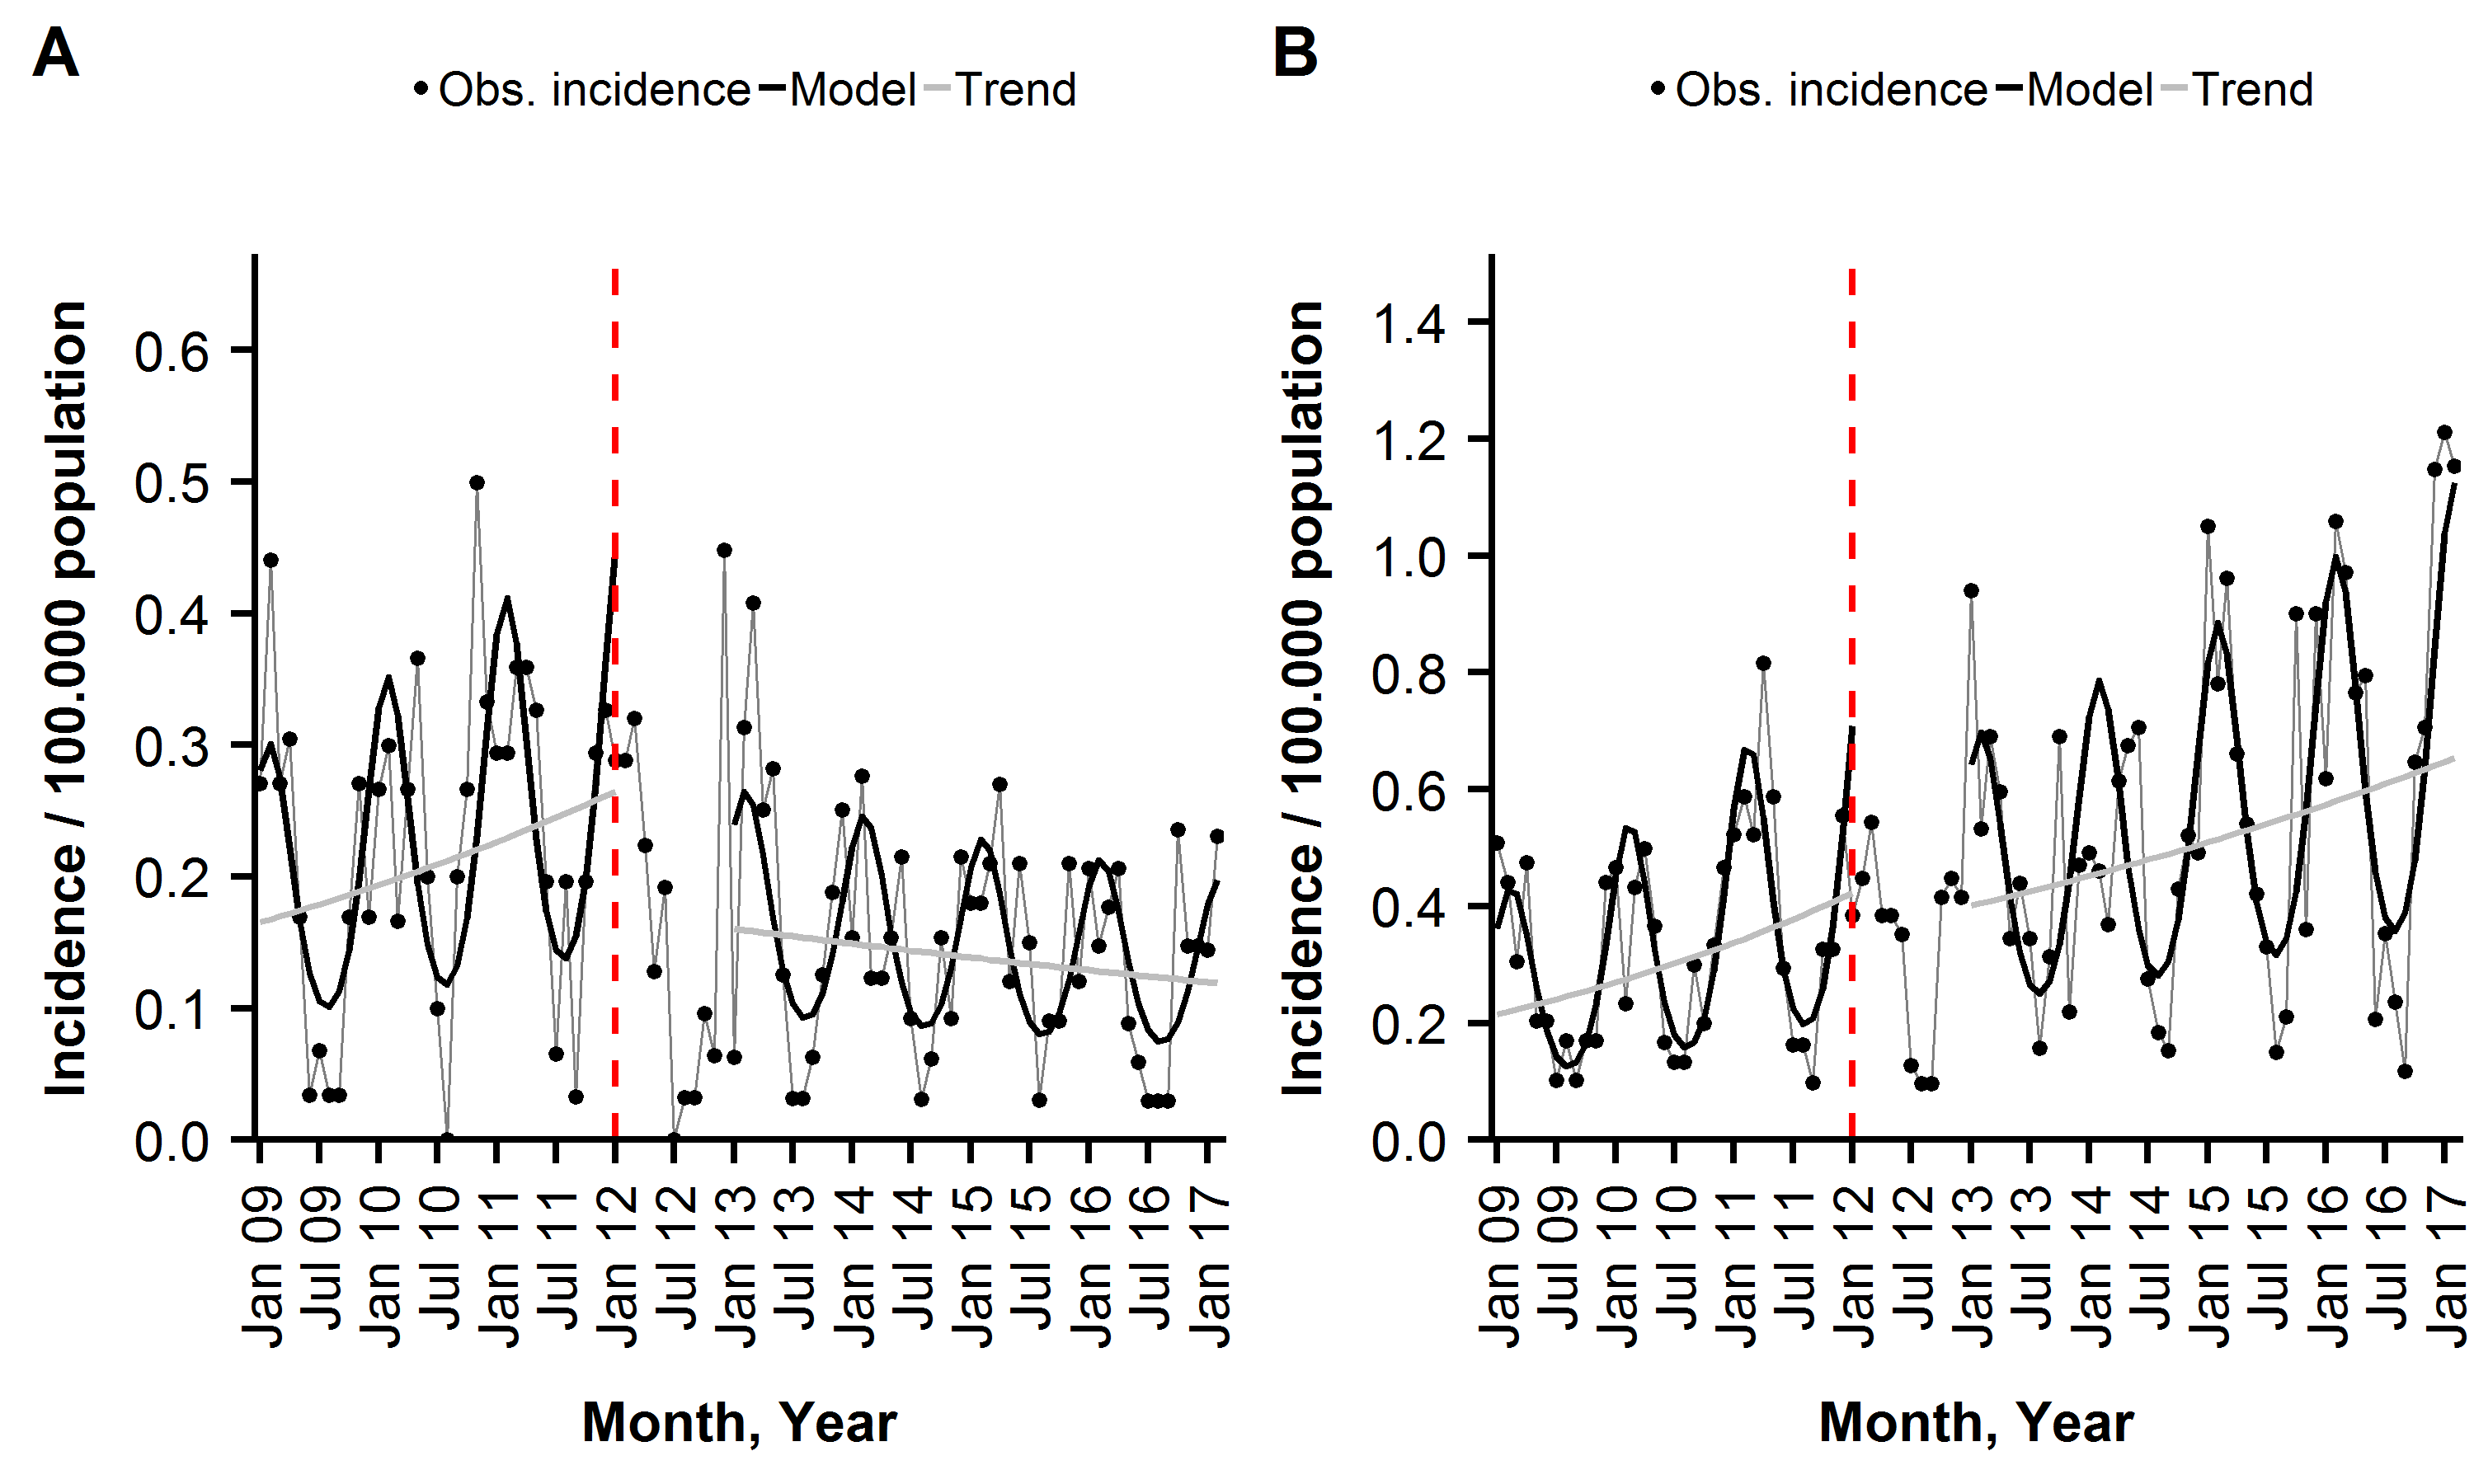
\includegraphics[width=\textwidth,height=0.5\textheight,keepaspectratio]{richter2019_Fig3.png}
\end{figure}
\end{center}

\vfill
{\scriptsize Richter et al. 2019}
\end{frame}
%%%%%%%%%%%%%%%%%%%%%%%%%%%%%%%%%%%%%%%%%%%%%%

%%%%%%%%%%%%%%%%%%%%%%%%%%%%%%%%%%%%%%%%%%%%%%
\begin{frame}[fragile]{IPD2}

\begin{block}{Model}
\begin{align*}
\begin{split}
\Log{Y_t}\, =
  &\, \Log{\mli{pop}_t} + \beta_0+\beta_1\,t + \beta_2\,\Sin{\frac{2 \pi t}{12}} \\
  &+ \beta_3\,\Cos{\frac{2 \pi t}{12}} + \beta_5\,\left(t-t_0\right)^+ \\
  &+\, \mathbbm{1}_{t-t_0>0} \left[\beta_4 + \beta_6\,\sin\left(\frac{2 \pi t}{12}\right) + \,\beta_7\,\cos\left(\frac{2 \pi t}{12}\right)\right]
\end{split}
\end{align*}

with
\begin{align*} 
(x)^+ = 
\begin{cases}
x, &\text{if $x > 0$,}\\
0, &\text{otherwise.}
\end{cases}
\end{align*}
\end{block}

\end{frame}
%%%%%%%%%%%%%%%%%%%%%%%%%%%%%%%%%%%%%%%%%%%%%%

%%%%%%%%%%%%%%%%%%%%%%%%%%%%%%%%%%%%%%%%%%%%%%
\begin{frame}[fragile]{Zika~\cite{ferguson2016}} % source: https://www.reconlearn.org/post/practical-vbd.html
Humans:
\begin{align*}
\frac{dS_h}{dt} &= \mu_h N_h - \frac {\beta_h b}{N_h} S_h  I_v - \mu_h  S_h \\
\frac{dI_h}{dt} &= \frac {\beta_h b}{N_h}S_h I_v - (\gamma_h + \mu_h) I_h \\
\frac{dR_h}{dt} &= \gamma_h I_h  - \mu_h I_h
\end{align*}

Vectors:
\begin{align*}
\frac{dS_v}{dt} &= \mu_v N_v  - \frac{\beta_v b} {N_h} I_h S_v - \mu_v S_v \\
\frac{dE_v}{dt} &= \frac{\beta_v b} {N_h} I_h S_v - (\delta + \mu_v) E_v \\
\frac{dI_v}{dt} &= \delta E_v - \mu_v I_v
\end{align*}
\end{frame}
%%%%%%%%%%%%%%%%%%%%%%%%%%%%%%%%%%%%%%%%%%%%%%

%%%%%%%%%%%%%%%%%%%%%%%%%%%%%%%%%%%%%%%%%%%%%%
\begin{frame}[fragile]{Zika2} % source: https://www.reconlearn.org/post/practical-vbd.html
\begin{knitrout}\scriptsize
\definecolor{shadecolor}{rgb}{0.969, 0.969, 0.969}\color{fgcolor}\begin{kframe}
\begin{alltt}
Lv       <-        \hlcom{# life span of \hlkwd{mosquitos} (in days)}
Lh       <-        \hlcom{# life span of \hlkwd{humans} (in days)}
Iph      <-        \hlcom{# Infectious period in \hlkwd{humans} (in days)}
IP       <-        \hlcom{# Infectious period in \hlkwd{vectors} (in days)}
EIP      <-        \hlcom{# Extrinsic incubation period in adult mosquitos}
muv      <-        \hlcom{# mortality of mosquitos}
muh      <-        \hlcom{# mortality of humans}
gamma    <-        \hlcom{# recovery rate in humans}
delta    <-        \hlcom{# extrinsic incubation rate}
b        <-        \hlcom{# Biting Rate}
betah    <-        \hlcom{# Probability of transmission from vector to host}
betav    <-        \hlcom{# Probability of transmission from host to vector}
Nh       <-        \hlcom{# Number of \hlkwd{humans} (Population of Cali 2.4 million)}
m        <-        \hlcom{# Vector to human ratio}
Nv       <-        \hlcom{# Number of vectors}
R0       <-        \hlcom{# Reproductive number}
b        <-        \hlkwd{sqrt}((R0 ^2 * muv*(muv+delta) * (muh+gamma)) /
                   (m * betah * betav * delta)) \hlcom{# biting rate}

TIME     <-        \hlcom{# Number of years to run the simulation for }
\end{alltt}
\end{kframe}
\end{knitrout}

\end{frame}
%%%%%%%%%%%%%%%%%%%%%%%%%%%%%%%%%%%%%%%%%%%%%%

%%%%%%%%%%%%%%%%%%%%%%%%%%%%%%%%%%%%%%%%%%%%%%
\begin{frame}[fragile]{Zika3} % source: https://www.reconlearn.org/post/practical-vbd.html

$S_h$: Susceptible Humans \\
$I_h$ : Infected/Infectious humans \\
$R_h$: Humans recovered from infection (with lifelong immunity) \\
$S_v$: Susceptible vectors \\
$E_v$: Exposed vectors 

\end{frame}
%%%%%%%%%%%%%%%%%%%%%%%%%%%%%%%%%%%%%%%%%%%%%%

%%%%%%%%%%%%%%%%%%%%%%%%%%%%%%%%%%%%%%%%%%%%%%
\begin{frame}[fragile]{GO ??}
a
\end{frame}
%%%%%%%%%%%%%%%%%%%%%%%%%%%%%%%%%%%%%%%%%%%%%%


%%%%%%%%%%%%%%%%%%%%%%%%%%%%%%%%%%%%%%%%%%%%%%
\begin{frame}[fragile]{Conclusion}
Here comes the conclusion
\end{frame}
%%%%%%%%%%%%%%%%%%%%%%%%%%%%%%%%%%%%%%%%%%%%%%



%%%%%%%%%%%%%%%%%%%%%%%%%%%%%%%%%%%%%%%%%%%%%%
\begin{frame}[fragile]{}
\begin{center}
\Huge{\textbf{Thank you!}}\\
\Huge{\textbf{Any questions?}}
\end{center}
\end{frame}
%%%%%%%%%%%%%%%%%%%%%%%%%%%%%%%%%%%%%%%%%%%%%%

\nocite{polonsky2019}
\nocite{richter2019}

\renewcommand*{\bibfont}{\scriptsize}
\setbeamertemplate{bibliography item}{\insertbiblabel}

\section{References}
%%%%%%%%%%%%%%%%%%%%%%%%%%%%%%%%%%%%%%%%%%%%%%
{\unnumbered
\begin{frame}[noframenumbering]
  \printbibliography
\end{frame}}
%%%%%%%%%%%%%%%%%%%%%%%%%%%%%%%%%%%%%%%%%%%%%%


\end{document}


